\section{N+1 view model}

N + 1 view modellen bruges til at beskrive software fra forskellige views. Modellen tager altid udgangspunkt i et use case view. Derefter er det op til udviklerholdet at bestemme hvor mange views der skal bruges for at beskrive systemet på tilstrækkelig vis. Til beskrivelse af dette system anvendes en 5 + 1 view model. På figur \ref{fig:5 + 1 view model} vises den anvendte model


\vspace{-5pt}
\begin{figure}[H]
	\centering
	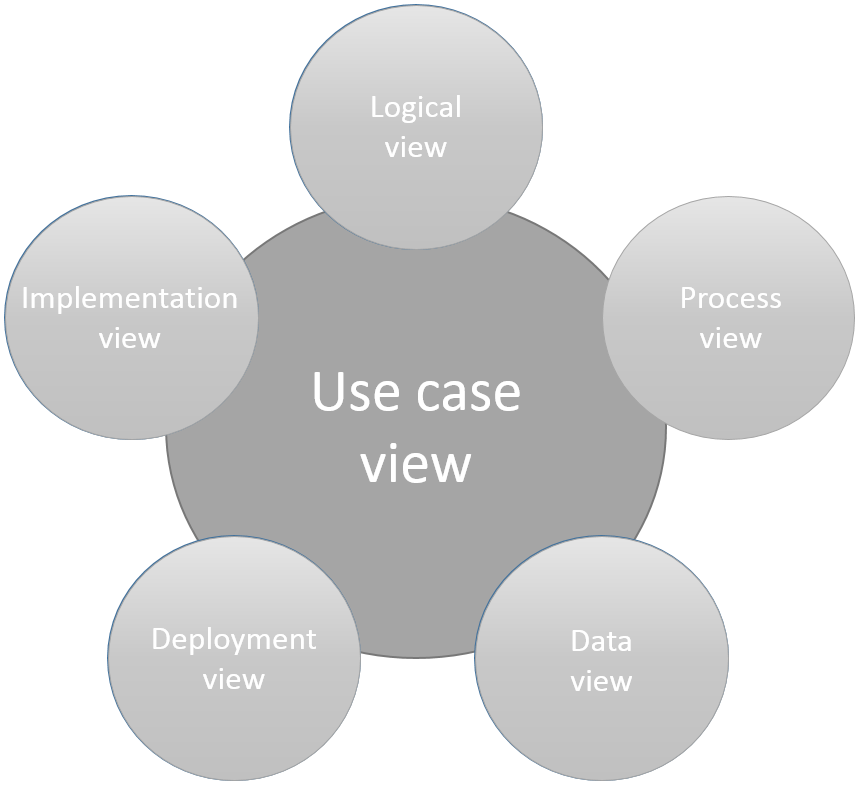
\includegraphics[width=0.7\textwidth]{Billeder/n+1}
	\vspace{0cm}
	\caption{5 + 1 view model}
	\label{fig:5 + 1 view model}
\end{figure}


\newpage

\subsection{View beskrivelse}

\textbf{Use case view}\\
Use case viewet består af use case beskrivelser, der er udviklet ud fra brugers synspunkt og som bruges til at beskrive systemets forskellige brugsscenarier. Alle udarbejdede use case beskrivelser forefindes i kravspecifikationen.

\textbf{Logical view}\\
Logical viewet bygges op af følgende fem diagrammer: Designoverview, pakke-, sekvens-, klasse- og state machine diagrammer.
Først udformes designoverview. Dernæst laves pakke og sekvensdiagrammer, og når de er udformet laves klassediagrammer. Til sidst udarbejdes state machines, som bruges til at beskrive flow mellem forskellige states.

\textbf{Process view}\\
Process viewet beskriver de forskellige processer/tråde i systemet og hvordan samspillet imellem disse er. Primært beskrives sammenspil mellem processer eller tråde der kører sideløbende med hinanden.

\textbf{Data view}\\
I data viewet beskrives layout af data der gemmes og hvordan det lagres. Desuden beskrives hvordan data sendes rundt i systemet og hvordan serverens database tilgås. 

\textbf{Deployment view}\\
I deployment viewet vises hvilke software pakker der bruges i systemet og hvor de bruges. Desuden beskrives hvilke protokoller der er anvendt i systemet, fx. layout af meddelelser med header/start/stop. 
  

\textbf{Implementation view}\\
I implementation viewet vises og beskrives hvilke værktøjer der er benyttet til projektet og hvordan disse værktøjer er sat op. Det beskrives også hvilke filer systemet er bygget af og hvordan disse filer skal linkes sammen. 
Desuden beskrives elementer som uden forklaring, ville være svære at forstå og bruge for udefrakommende. Målet med implementation viewet er at gøre det klart hvordan projektet er udarbejdet, og derved gøre det muligt for udefrakommende at genoptage arbejde på projektet.


